\documentclass[tikz, border=10pt]{standalone}
\usepackage{circuitikz}
\usetikzlibrary{shapes, arrows, positioning, calc}

\begin{document}

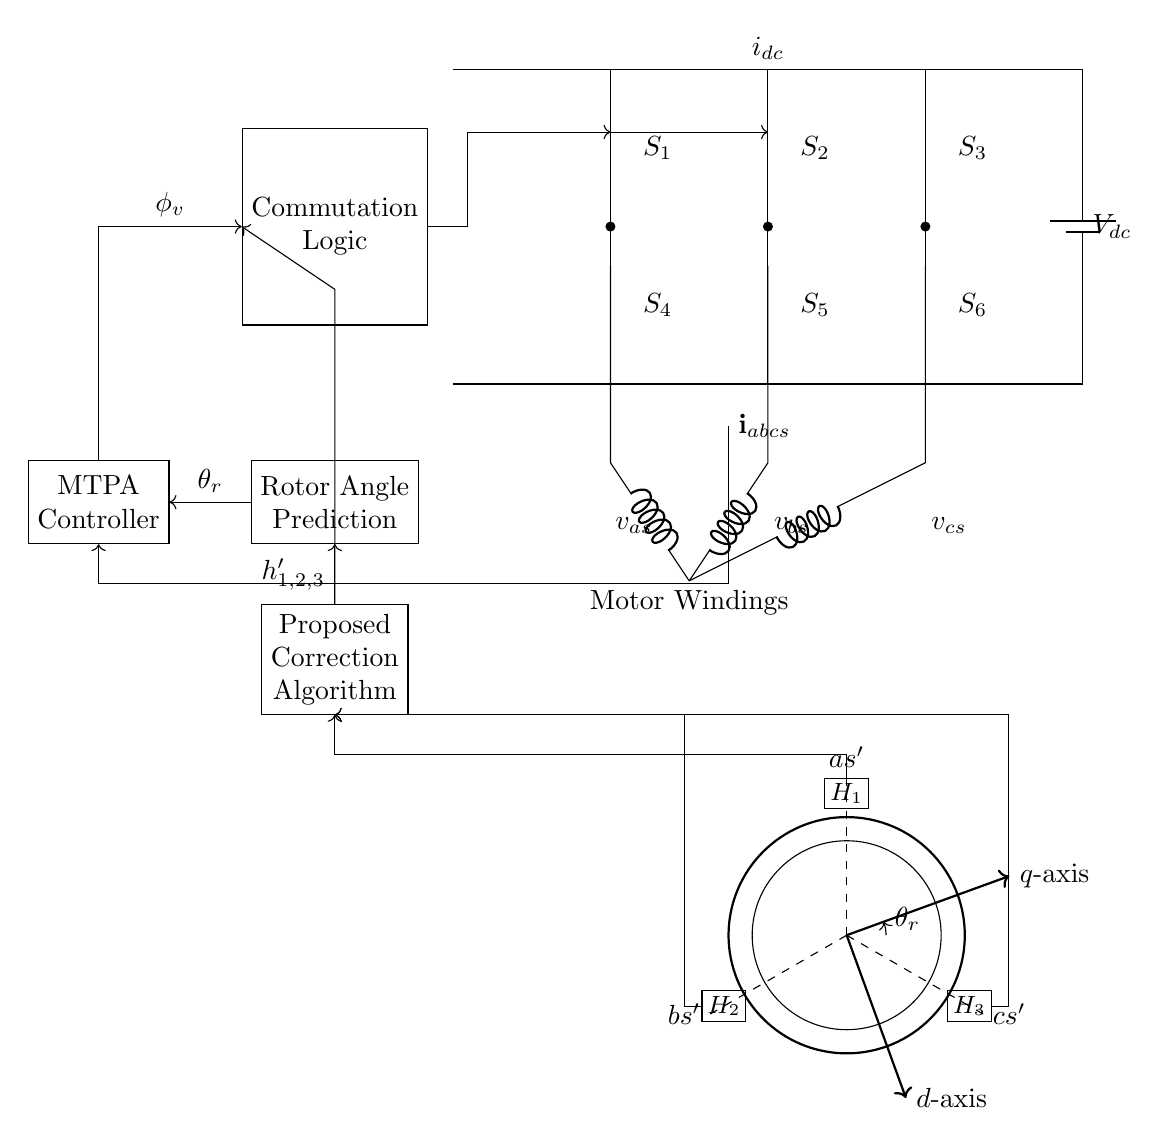
\begin{tikzpicture}[
    block/.style={draw, fill=white, rectangle, minimum height=3em, minimum width=4em, align=center},
    sum/.style={draw, fill=white, circle, node distance=1cm},
    input/.style={coordinate},
    output/.style={coordinate},
    pinstyle/.style={pin edge={to-,thin,black}}
]

% --- 1. THE INVERTER (Top) ---
% DC Bus
% We use explicit nodes for labels to avoid package errors
\draw (-2,5) -- (6,5);
\node[above] at (2, 5) {$i_{dc}$}; % Manual label for current
\draw (6,5) to[battery1] (6,1);
\node[right] at (6, 3) {$V_{dc}$}; % Manual label for Voltage
\draw (-2,1) -- (6,1);

% Inverter Legs
% We strip all fancy attributes and just draw the component
% Leg A
\draw (0,5) to[nigbt] (0,3) to[nigbt] (0,1);
\node at (0.6, 4) {$S_1$}; % Manually placed text
\node at (0.6, 2) {$S_4$};
\draw (0,3) to[short, *-] (0,2.5) coordinate (PhA_out);

% Leg B
\draw (2,5) to[nigbt] (2,3) to[nigbt] (2,1);
\node at (2.6, 4) {$S_2$};
\node at (2.6, 2) {$S_5$};
\draw (2,3) to[short, *-] (2,2.5) coordinate (PhB_out);

% Leg C
\draw (4,5) to[nigbt] (4,3) to[nigbt] (4,1);
\node at (4.6, 4) {$S_3$};
\node at (4.6, 2) {$S_6$};
\draw (4,3) to[short, *-] (4,2.5) coordinate (PhC_out);

% --- 2. CONTROL BLOCKS (Left Side) ---
\node [block, minimum height=2.5cm, minimum width=1.5cm] (logic) at (-3.5, 3) {Commutation\\Logic};

% Connections from Logic to Gates
\draw[->] (logic.east) -- ++(0.5,0) |- (-0.5, 4.2) -- (0, 4.2); % S1
\draw[->] (logic.east) -- ++(0.5,0) |- (1.5, 4.2) -- (2, 4.2); % S2

\node [block] (pred) at (-3.5, -0.5) {Rotor Angle\\Prediction};
\node [block] (corr) at (-3.5, -2.5) {Proposed\\Correction\\Algorithm};

% MTPA Controller (Left)
\node [block, align=center] (mtpa) at (-6.5, -0.5) {MTPA\\Controller};

% --- 3. SIGNAL FLOW ---
\draw[->] (mtpa.north) |- node[above, near end] {$\phi_v$} (logic.west);
\draw[->] (pred.west) -- node[above] {$\theta_r$} (mtpa.east);
\draw[<-] (mtpa.south) -- ++(0,-0.5) -- ++(8,0) -- ++(0,2) node[right] {$\mathbf{i}_{abcs}$};

% Hall Signals
\draw[->] (corr.north) -- node[left] {$h'_{1,2,3}$} (pred.south);
\draw[->] (corr.north) -- ++(0, 4) -- (logic.west); 

% --- 4. MOTOR WINDINGS ---
\draw (PhA_out) -- (0,0) to[L] (1,-1.5);
\draw (PhB_out) -- (2,0) to[L] (1,-1.5); 
\draw (PhC_out) -- (4,0) to[L] (1,-1.5);
\node at (1,-1.5) [below] {Motor Windings};

% Manual labels for inductors
\node at (0.3, -0.8) {$v_{as}$};
\node at (2.3, -0.8) {$v_{bs}$};
\node at (4.3, -0.8) {$v_{cs}$};


% --- 5. MOTOR CROSS SECTION ---
\begin{scope}[shift={(3,-6)}] 
    \draw[thick] (0,0) circle (1.5cm); 
    \draw (0,0) circle (1.2cm); 

    \draw[dashed] (0,0) -- (90:2cm) node[above] {$as'$};
    \draw[dashed] (0,0) -- (210:2cm) node[left] {$bs'$};
    \draw[dashed] (0,0) -- (330:2cm) node[right] {$cs'$};

    \draw[->, thick] (0,0) -- (290:2.2cm) node[right] {$d$-axis};
    \draw[->, thick] (0,0) -- (20:2.2cm) node[right] {$q$-axis};

    \node[draw, rectangle, inner sep=2pt] (H1) at (90:1.8cm) {\small $H_1$};
    \node[draw, rectangle, inner sep=2pt] (H2) at (210:1.8cm) {\small $H_2$};
    \node[draw, rectangle, inner sep=2pt] (H3) at (330:1.8cm) {\small $H_3$};
    
    \draw[->] (H1) -- ++(0,0.5) -| (corr.south);
    \draw[->] (H2) -- ++(-0.5,0) |- (corr.south);
    \draw[->] (H3) -- ++(0.5,0) |- (corr.south);
    
    \draw[->] (0.5,0) arc (0:20:0.5);
    \node at (15:0.8) {$\theta_r$};
\end{scope}

\end{tikzpicture}
\end{document}